\section{Design Overview}
\label{sec:overview}

\sys is a compilation and runtime system for skills.
It makes skills portable across heterogeneous targets by
combining an AOT compiler~\cite{aho2006compilers} that specializes skills at install time
with a runtime that resolves execution-time uncertainty.
Figure~\ref{fig:overview} shows the architecture.

\begin{figure}[t]
  \centering
  \setlength{\belowcaptionskip}{-10pt}
  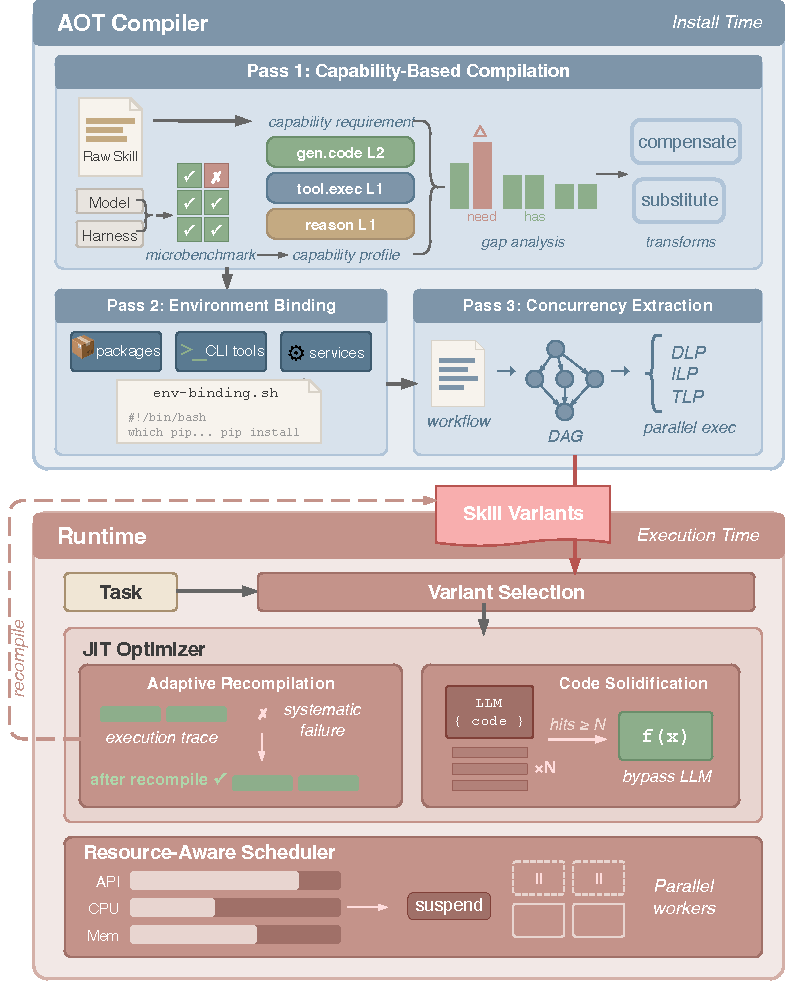
\includegraphics[width=\columnwidth]{figures/skillos_overview.pdf}
  \caption{\sys architecture. The AOT compiler produces
    optimized skill variants at install time through three
    passes. The runtime manages variant selection, JIT
    optimization, and resource-aware scheduling during
    execution.}
  \label{fig:overview}
\end{figure}

\heading{AOT Compiler.}
At skill installation time, the compiler analyzes the
skill against the target environment and produces one or more optimized
\emph{skill variants}. The compiler performs three distinct passes:
\emph{Capability-based compilation}
(\S\ref{sec:compiler:cap}) handles model and harness
mismatch (P1--P2) by adapting the skill to the target's
available capabilities.
\emph{Environment binding}
(\S\ref{sec:compiler:env}) handles environment mismatch
(P3) by materializing the dependencies required for
execution.
\emph{Concurrency extraction}
(\S\ref{sec:compiler:par}) identifies parallelism latent in
the skill's workflow and maps it to the target harness.
Compiled variants are stored per target.

\heading{Runtime \& JIT optimizer.}
When a task arrives, the runtime selects the variant
compiled for the current (model, harness) pair and loads
it through the standard progressive disclosure mechanism.
Two components then operate on top of normal execution.
The \emph{JIT optimizer} (\S\ref{sec:runtime:jit})
monitors execution outcomes across invocations and
triggers recompilation when it detects capability gaps
that the AOT compiler missed.
It also compiles structurally fixed code patterns into
executable functions that bypass the LLM inference entirely.
The \emph{resource-aware scheduler}
(\S\ref{sec:runtime:sched}) bridges compile-time
parallelism annotations and run-time resource availability,
throttling or suspending concurrent sub-agents when
demand exceeds capacity.
